\begin{figure}[h]
 \centering
 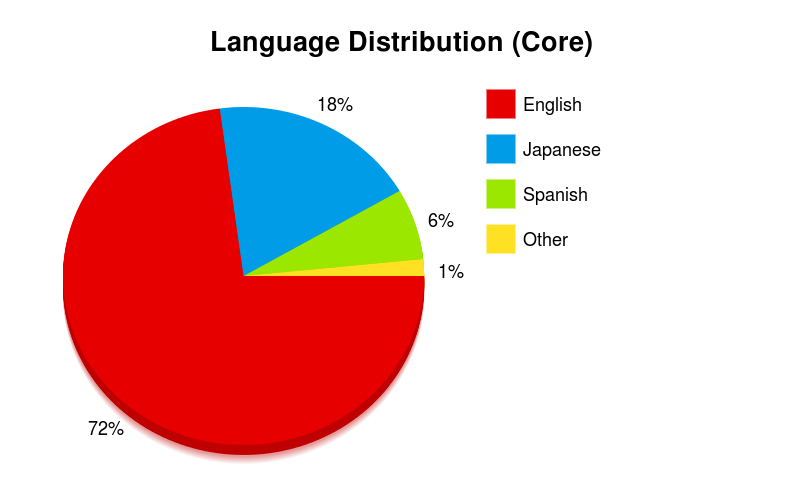
\includegraphics[bb=0 0 800 500,scale=.2]{./images/lang-core.png}
 % lang-core.png: 800x500 pixel, 72dpi, 28.22x17.64 cm, bb=0 0 800 500
 \caption{For the core set, the percentage users who have marked Japanese as their Twitter language is more than four times that of the random set.}
\label{fig:lang-core}
\end{figure}

\begin{figure}[h]
 \centering
 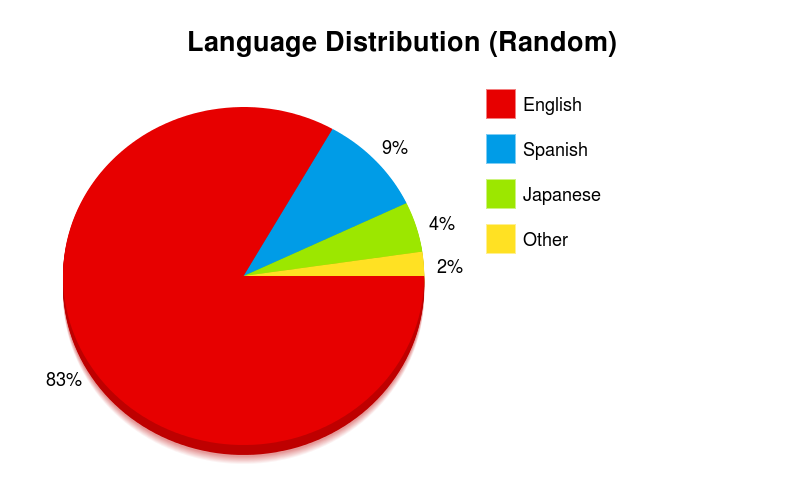
\includegraphics[bb=0 0 800 500,scale=.2]{./images/lang-rand.png}
  % lang-rand.png: 800x500 pixel, 72dpi, 28.22x17.64 cm, bb=0 0 800 500
 \caption{English, Spanish, and Japanese are the top languages for both the connected and the random user sets.}
\label{fig:lang-rand}
\end{figure}

\begin{figure}[t]
 \centering
 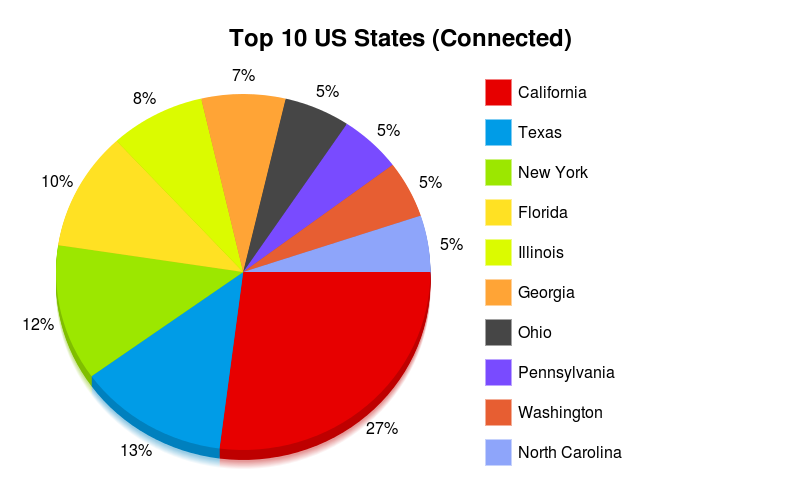
\includegraphics[bb=0 0 800 500,scale=.2]{./images/loca-conn.png}
 % loca-conn.png: 800x500 pixel, 72dpi, 28.22x17.64 cm, bb=0 0 800 500
\caption{}
\label{fig:loca-conn}
%\end{figure}

%\begin{figure}
% \centering
 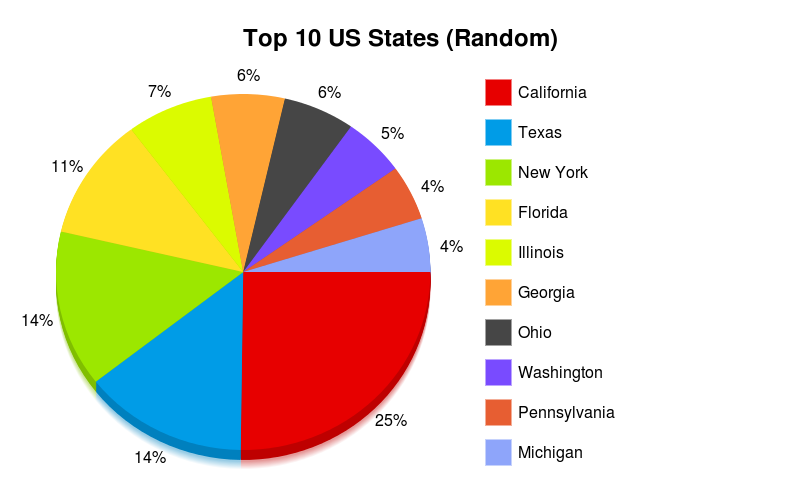
\includegraphics[bb=0 0 800 500,scale=.2]{./images/loca-rand.png}
 % loca-rand.png: 800x500 pixel, 72dpi, 28.22x17.64 cm, bb=0 0 800 500
\caption{}
\label{fig:loca-rand}
%\end{figure}

%\begin{figure}
% \centering
 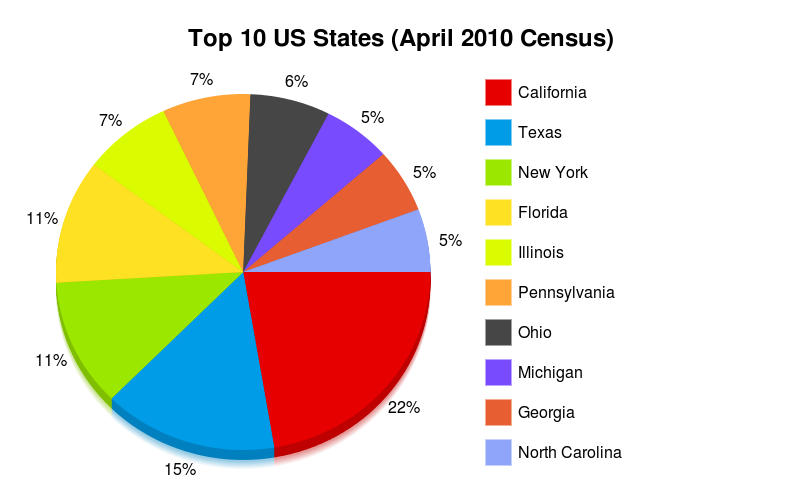
\includegraphics[bb=0 0 800 500,scale=.2]{./images/loca-actu.png}
 % loca-actu.png: 800x500 pixel, 72dpi, 28.22x17.64 cm, bb=0 0 800 500
\caption{The distribution of U.S. states for both the random and the connected datasets aligns well with the population census data.}
\label{fig:loca-actu}
\end{figure}

At the start of our work we inherited a large dataset from Rejaie \textit{et all} that was created through a biased sampling of the Twitter network.  The dataset contained partial connectivity information for 242,275 potentially influential users.  Due to limitations of the Twitter REST API at the time of collection, the connectivity data was incomplete.  Additionally, the dataset did not include the associated attribute information for each user because it was not germane to Rejaie's previous work.  This dataset needed to be completed before beginning our analysis.

Our goal was to characterize the relationships in a completed section of the Twitter network.  It was first necessary to determine if a large, complete subgraph existed within this dataset.  A collection of smaller subgraphs would not be sufficient as they would be less likely to capture the impact of rare influential users.  By performing a series of reconstructions of the graphs in the dataset we were able to discover a single subgraph of 215,606 sampled users.  Including the next hop information for these sampled users, the subgraph included 16 million unique user accounts.

The inherited dataset was not originally intended to measure the extreme connectivity degrees of rare users.  As a result, the friend and follower information for each user in the subgraph were truncated at 1,000 connections apiece.  This truncation was due to the prohibitive rate limiting of of the Twitter API, which made it infeasible to collect the complete connectivity information for these users in real time.  Over the course of several weeks we were able to restore this missing information, growing our subgraph to the inclusion of over 30 million unique users.  Several months passed between these two collection phases.  The potential error that this introduced is explored below.

Simultaneously, we needed to collect the user attribute information for the tens of millions of users in our subgraph.  Completing this task via the Twitter API was difficult due to the connectivity restoration process, and it was not our wish to violate Twitter's terms of service by launching API calls from dozens of hosts.  Fortunately, we were able to find an alternate method of collecting user attribute information.  Twitter provides XML dumps of user information through their primary website.  These calls are not subject to API rate limites, presumably for the benefit of mobile applications that may issue frequent user lookups.  Using this service, we were able to collect the necessary information without violating the Twitter API ToS.

\subsection{Measuring Error}

Because our user attribute information was collected in less than a month, we have assumed that no significant error is present.  It is not possible to capture a realtime snapshot of user attributes in the Twitter network, so we have no method of comparing collected attributes to actual attributes.  Our intuition here is that most user attributes are not subject to frequent change.  The exception to this is connectivity, which is explored below.  For our purposes, the collected user attribute information can be accepted as accurate.

In contrast, connectivity information for our subgraph was collected in two different phases between September 2010 and February 2011.  It would be foolish to assume that significant change did not occur in the network over this time.  It was therefore necessary to confirm that the temporally disparate collection phases did not introduce error to our network measurements.  To do this, we compared our snapshot of connectivity for each user to the stated connectivity in each user's attributes.

\begin{figure}
 \centering
 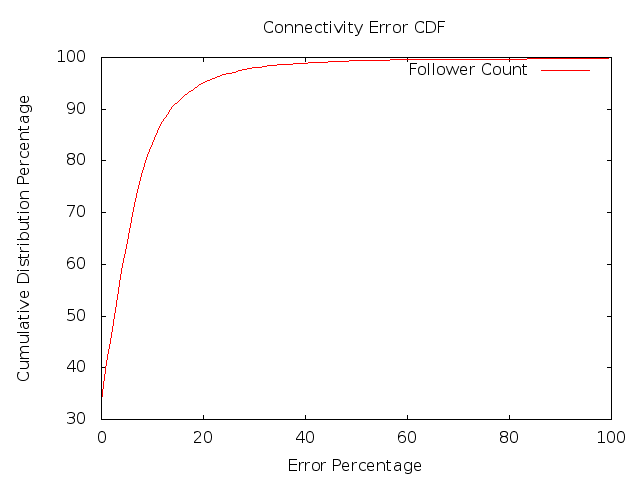
\includegraphics[bb=0 0 640 480,scale=.3]{./images/Bates-Final/CDF.png}
 % CDF.png: 640x480 pixel, 72dpi, 22.58x16.93 cm, bb=0 0 640 480
 \label{fig:cdf}
\end{figure}

Figures \ref{cdf} confirms that we have captured an accurate view of connectivity in our piece of the Twitter network.  90\% of users have a follower count error of less than 15\%.  Most users that exhibit a non-negligible error percentage are of a very low degree, and are therefore not of high significance in our subgraph.  High degree users exhibited the lowest error rate because their connectivity information was collected most recently.  This holds true for friend count as well.  It is our belief that our connectivity error is sufficiently low that are results are meaningful.

\subsection{Profiling}

Our set of Twitter users was created by first discovering the IDs of approximately 250,000 users that met a certain time-in-system threshold, and then querying the Twitter API for all users connected to that initial core.  Since user connectivity is central to our study, this allowed us to quickly acquire a subgraph in which every node was usable.  However, since this collection method was not random, the distribution of attributes across our dataset could be different than that which we would observe by choosing random users.  These differences are important to examine because they may indicate ways that our dataset is not generalizable to the entire Twitter universe.

To quantify these potential discrepancies, we performed attribute profiling for both our connected subgraph and a set of 1.5 million randomly-selected users.  We calculated the percentages of users falling into each attribute grouping for each set and then compared the two profiles.  We also contrasted the profiles of the core users in our subgraph to the other connected, next-hop users.

\subsubsection{Boolean Attributes}

Two of the attributes we examined were true/false values: protected and geo-enabled.  Below is a table of percentages of users who enabled each attribute, for the core, connected, and random data sets.

\begin{center}
\begin{tabular}{| l | r | r | r |}
\hline
\textbf{Attribute} & \textbf{Core} & \textbf{Connected} & \textbf{Random} \\ \hline
Protected & 3.6 & 12.3 & 8.3 \\ \hline
Geo-Enabled & 24.5 & 15.8 & 6.7 \\ \hline
Verified & 0.1 & 0.0 & 0.0 \\ \hline
Contributors Enabled & 0.0 & 0.0 & 0.0 \\ \hline
Show All Inline Media & 7.9 & 6.3 & 1.6 \\ \hline
URL & 49.7 & 26.7 & 10.2 \\ \hline
Is Translator & 0.0 & 0.0 & 0.0 \\ \hline
\end{tabular}
\end{center}
\textit{Attribute distribution percentages for three data sets.}\\

We found that our core users were less than half as likely to be protected, and more than three times more likely to allow the inclusion of GPS information in their tweets than the random users.  The percentage of geo-enabled users in the connected subgraph is in between that of core and random, which indicates that the original user selection could have carried over to the first-hop connections to some extent.  Interestingly, the subgraph users are more likely than either of the other sets to be protected.  This may be because users who are connected to the initial group, which we would characterize as more ``established", are more experienced than the average random user, as random users likely include many people who have signed up but have not made much use of their accounts.  The random set could, for example, include users who are not connected to anyone else.

\subsubsection{Language}

Users have seven choices for the language attribute.  Choice of language affects the text of the Twitter interface, but does not translate tweets.  It is unclear whether the language changes based on the location (IP address) of the user, or if English is default for everyone.  We find that, in comparison to the random set, the connected and core users are substantially more likely to be configured for using Japanese (Figures \ref{fig:lang-core}, \ref{fig:lang-rand}).  This could indicate that the filtering techniques used to gather our original set of users was more likely to pick up Japanese users.

\begin{center}
\begin{tabular}{| l |  r | r | r |}
\hline
\textbf{Language} & \textbf{Core} & \textbf{Connected} & \textbf{Random} \\ \hline
English & 72.9 & 78.3 & 83.2 \\ \hline
Spanish & 6.8 & 12.1 & 9.7 \\ \hline
Japanese & 18.7 & 7.6 & 4.8 \\ \hline
French & 0.5 & 0.8 & 1.2 \\ \hline
German & 0.7 & 0.7 & 0.7 \\ \hline
Italian & 0.3 & 0.4 & 0.5 \\ \hline
Korean & 0.1 &  0.1 & 0.0 \\ \hline
\end{tabular}
\end{center}
\textit{Language distribution percentages for three data sets.}\\

\subsubsection{Location}

We examined data for the ten U.S. states with the greatest number of associated users.  Distribution of locations was similar between the connected and random sets, and also aligned fairly well with population data (Figures \ref{fig:loca-conn}, \ref{fig:loca-rand}, \ref{fig:loca-actu}).  For the states that appear in all three data sets, all percentages are within 5\% of each other, and most are differ by no more than 2\%.  Also, the top five states are the same and in the same order.

\subsection{Approaching Attribute Analysis}

\subsubsection{Location}

The location attribute field has no enforced format, apart from length.  That is, users can type in essentially any text for their location.  From a small random sample and manual examination of this attribute field, we estimate that approximately 50\% of users provide location text that can be matched to at least one city, state/region, or country.  We also find that almost 90\% of users who match one city will match more than one city.  Since we want our analyses to be by specific location, we need to address these ambiguities.

\begin{figure*}[t]
 \centering
 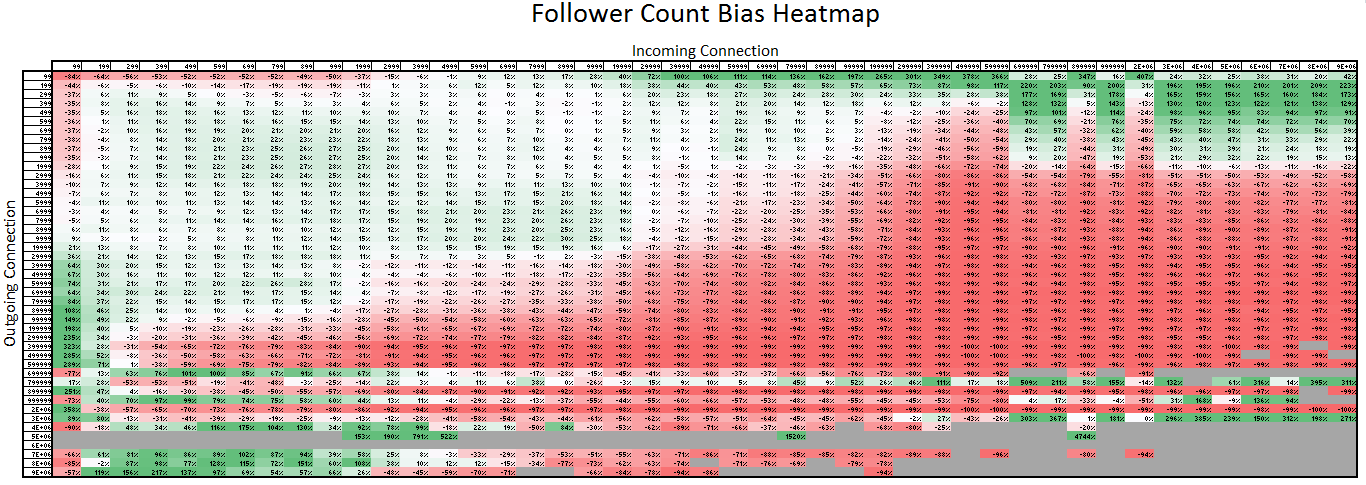
\includegraphics[bb=0 0 1025 364, scale=.4]{./images/Bates-Final/followercount.png}
 % followercount.png: 1366x485 pixel, 96dpi, 36.15x12.83 cm, bb=0 0 1025 364
 \label{fig:follower_count}
 \caption{A connectivity bias chart for number of followers in logarithmically increasing groupings.}
\end{figure*}

\begin{figure*}[t]
 \centering
 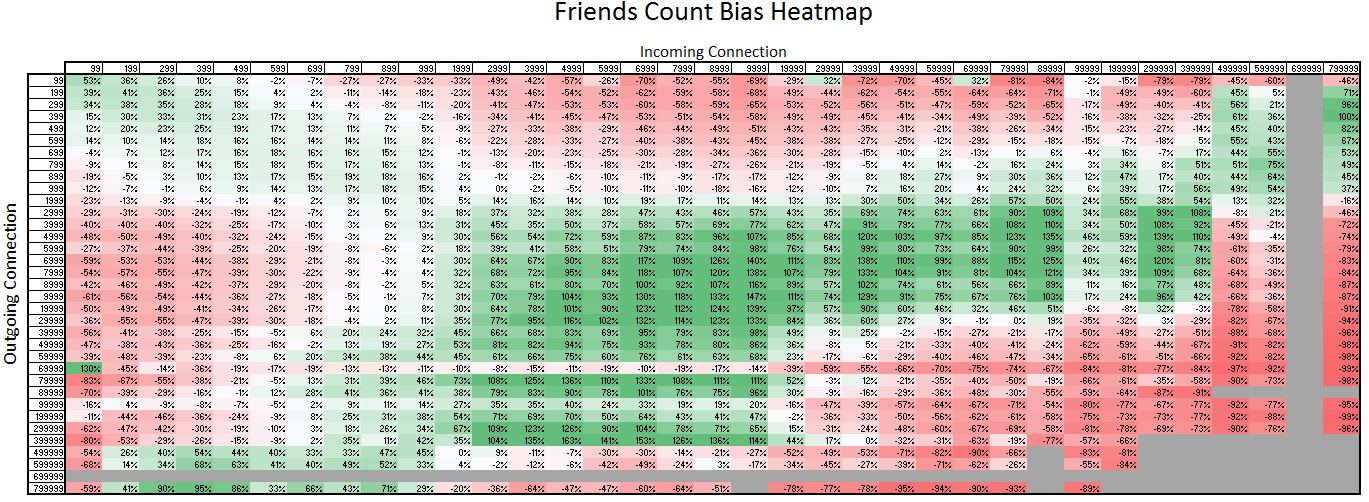
\includegraphics[bb=0 0 1027 377, scale=.4]{./images/Bates-Final/friendscount.png}
 % friendscount.png: 1369x502 pixel, 96dpi, 36.23x13.28 cm, bb=0 0 1027 377
 \label{fig:friend_count}
 \caption{A connectivity bias chart for number of friends in logarithmically increasing groupings.}
\end{figure*}

Given that there are hundreds of thousands of cities in the world, we decided to start our location analyses with U.S. states because of their familiarity to the authors.  Our approach is to filter users based on exact matches with a pre-compiled list of U.S. cities in the standard \textit{San Francisco, CA} or \textit{San Francisco, California} format.  If a user matches one of these locations exactly, the user cannot exactly match a different location.  For the top 100 most populous cities, we try to match the city name itself, without the state, with the intuition that, for example, users from \textit{San Francisco} would not find it necessary to specify their state.

We find that 8\% of connected users and 5\% of random users are successfully matched to a state.
